\documentclass[10pt,a4paper, openany]{book}
\usepackage[utf8]{inputenc}
\usepackage[english]{babel}
\usepackage{amsmath}
\usepackage{amsfonts}
\usepackage{amssymb}
\usepackage{graphicx}
\usepackage{color}
\usepackage{lmodern}
\usepackage{tablefootnote}
\usepackage[sc]{mathpazo}
\usepackage{booktabs}
\usepackage{hyperref}
\usepackage{fancyhdr}
\hypersetup{pdftex, colorlinks=true,linkcolor=black}

\usepackage{floatrow}
\newfloatcommand{capbtabbox}{table}[][\FBwidth]
\usepackage{blindtext}

\author{Armando Brandonisio}
\title{\textbf{Instrumental chapters}\\COMPASS thesis}

\begin{document}
\maketitle
\tableofcontents \newpage


\chapter{Absorber characterization}

Characterization of scintillator rods is a fundamental starting point to understand possibilities and limits of the entire experiment.\\
Absorber bars are the external objects of polarimeter design, and they must be made of a high atomic number $Z$ to maximize absorption of the radiation.\\
A good light yield and emission velocity ($\leq 1\mu s$) are recomended to optimize spectrum detection and coincidence measurements.\\
The agreement between absorber light emission spectrum and the photo-detection efficiency range of SiPM increases the collected charge of the readout process.\\
The measurements have been carried out by illuminating the scintillation rod with a X-ray beam.\\
$Si$PM and electronic chain parameters was varied measuring the relative position of the photo-peak in the spectrum produced by the scintillator.


\section{Absorber properties}
We investigated luminescence and scintillation properties of the $Gd_3 Al_2 Ga_3 O_{12} : Ce$ (GAGG) produced by \emph{Furukawa} company.\\
The GAGG crystal has the highest light yield among oxide crystal at room temperature \cite{abs:1} and fast decay time for the detection of radioactivity and in nuclear and particle physics experiments.\\
A list of the most important parameters for GAGG is reported in Table \ref{tab:abs1}.

\begin{table}[h]
\begin{tabular}{cccccccc}
\toprule
Density & Light & Decay & Peak & Energy & Hygroscopicity  \\
 $[g/cm^3]$ & yield & time & emission & resolution &   \\
   & [photon/MeV] & [ns] & [nm] & [\% @662 keV] &   \\
\midrule
6.63 & 57000 & 88 (91\%) & 520 & 5.2  & No\\
 & & 258 (9\%) & & & \\
\bottomrule
\end{tabular}
\caption{Physical and scintillation properties of GAGG (data from~\cite{gagg:1})} \label{tab:abs1}
\end{table}

Some fundamental features of this crystal are that it has no intrinsic radioactivity and it is a non-hygroscopic material. This allows a better usage for experimentation with low risk of contamination from ambient.\\[2ex]

We know all GAGG properties (Tab~\ref{tab:abs1}) and cross section values with respect to energy. Results value in Fig~\ref{fig:cs_gagg}.

\begin{figure}[!h]
\begin{center}
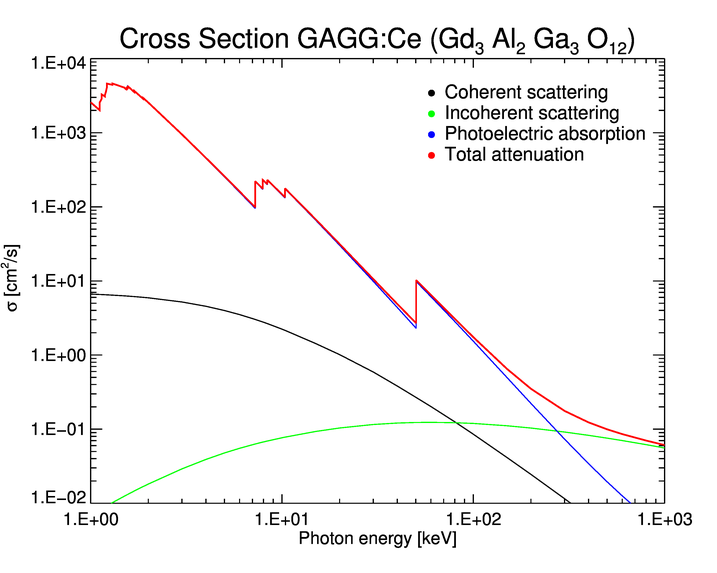
\includegraphics[scale=0.25]{imm/cs_gagg.png}
\end{center}
\caption{Mass attenuation coefficients for the GAGG crystal (Data from~\cite{gagg:2})}
\label{fig:cs_gagg}
\end{figure}
\begin{figure}[!h]
\begin{center}
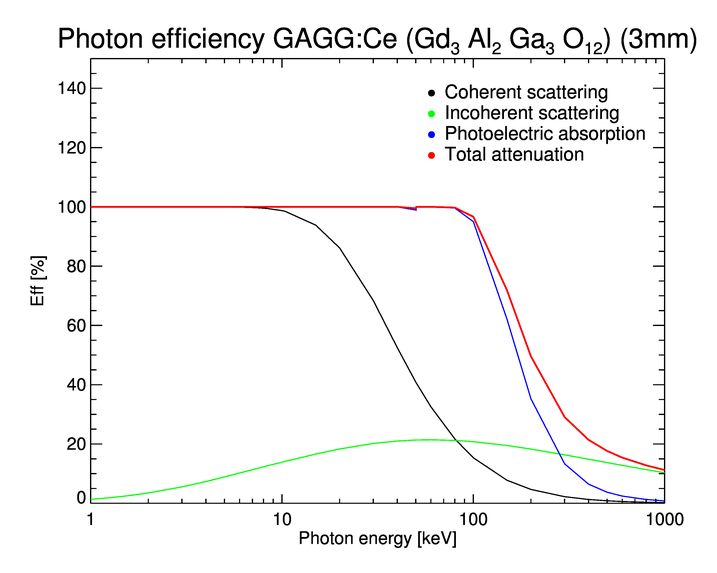
\includegraphics[scale=0.26]{imm/eff_gagg_3mm.png}
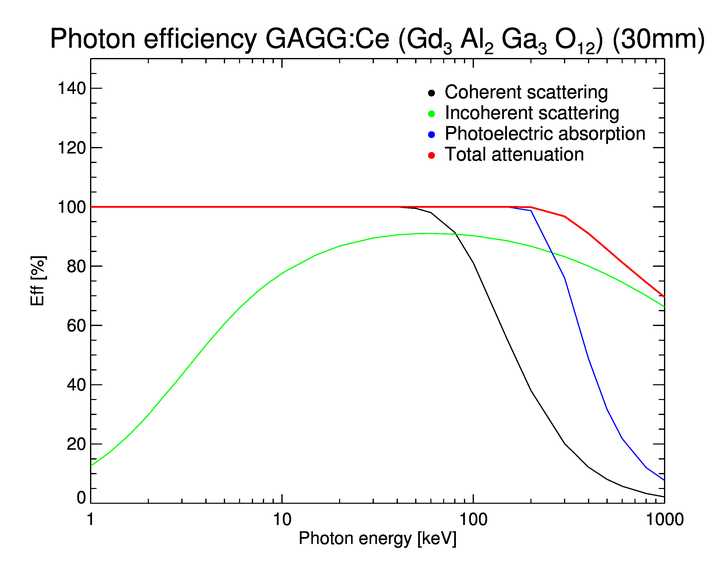
\includegraphics[scale=0.26]{imm/eff_gagg_30mm.png}
\end{center}
\caption{Total GAGG efficiency for a thickness of 3mm (left) and 30mm (right)}
\label{fig:eff_gagg}
\end{figure}


\section{Experimental set-up}
Laboratory measurements have been carried out using a single rod made of GAGG produced by \emph{Furukawa} company.\\
The rod has a square-base parallelepipoidale shape with a height of 30mm and a side of 3mm , thus their dimension results 2/3 lower  to the one expected for the polarimeter bars ($\sim 10mm$).\\
To minimize the loss of photons during scintillation, the bar was \emph{wrapped} with Teflon Fig~\ref{fig:gagg1}, that has a high light diffusion power.

\begin{figure}[!h]
\begin{center}
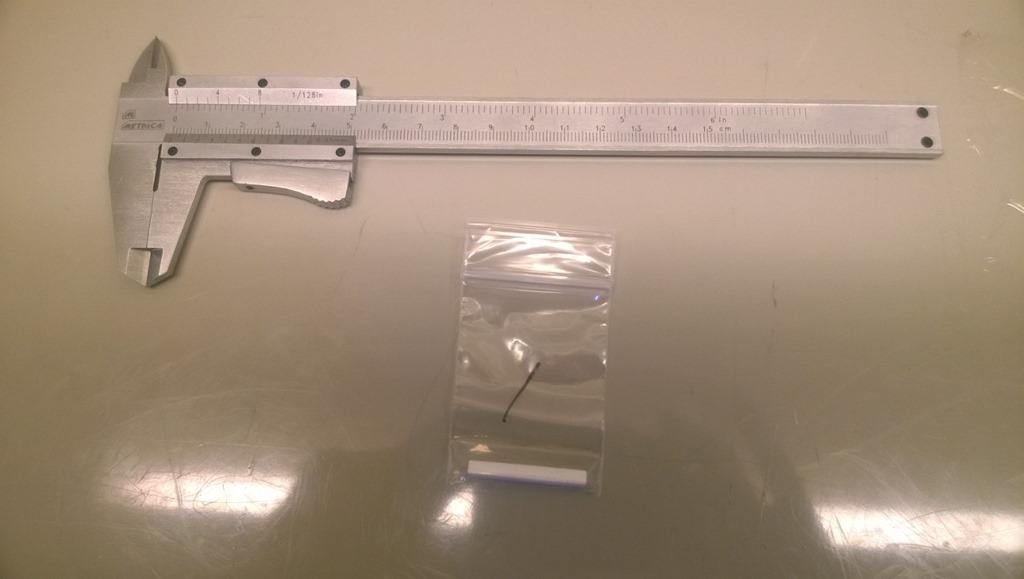
\includegraphics[scale=0.33]{imm/gagg1.jpg}
\end{center}
\caption{Scintillation rod made of GAGG wrapped with teflon}
\label{fig:gagg1}
\end{figure}

The rod has been placed over a single SiPM, models LCT4/9 and LCT5/1 produced by the Hamamatsu company.\\
Properties, CAD scheme and microscopic details of this SiPM are reported in Tab~\ref{tab:lct4}, Fig~\ref{fig:lct4_cad} and Fig~\ref{fig:lct4_1} respectively.

\begin{figure}[h]
\begin{floatrow}
\ffigbox{%
  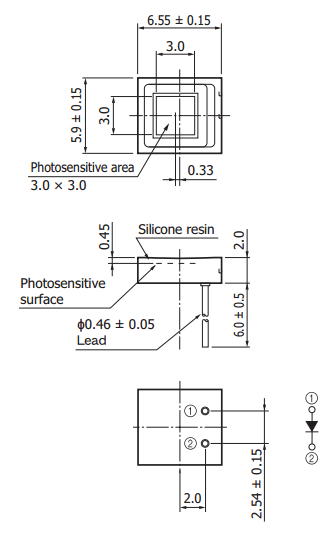
\includegraphics[scale=0.55]{imm/lct4_cad.png}%
}{%
  \caption{CAD scheme for LCT4/9 and LCT5/1}\label{fig:lct4_cad}%
}
\capbtabbox{%
\begin{tabular}{ll}
\textbf{LCT4/9} &\\
\toprule
Cell pitch & $75\mu m$ \\
Device size & $3\times 3mm^2$\\
Microcells & 1600\\
Surface coating & Silicone resin\\
Fill-factor & 73\% \\
Breakdown & 51.10 V\\
\bottomrule
 & \\
\textbf{LCT5/1} &\\
\toprule
Cell pitch & $50\mu m$ \\
Device size & $3\times 3mm^2$\\
Microcells & 3600\\
Surface coating & Silicone resin\\
Fill-factor & 74\% \\
Breakdown & 52.5 V\\
\bottomrule
\end{tabular}
}{%
  \caption{Main physical features of LCT/9 and LCT5/1}\label{tab:lct4}%
}
\end{floatrow}
\end{figure}

\newpage

\begin{figure}[!h]
\begin{center}
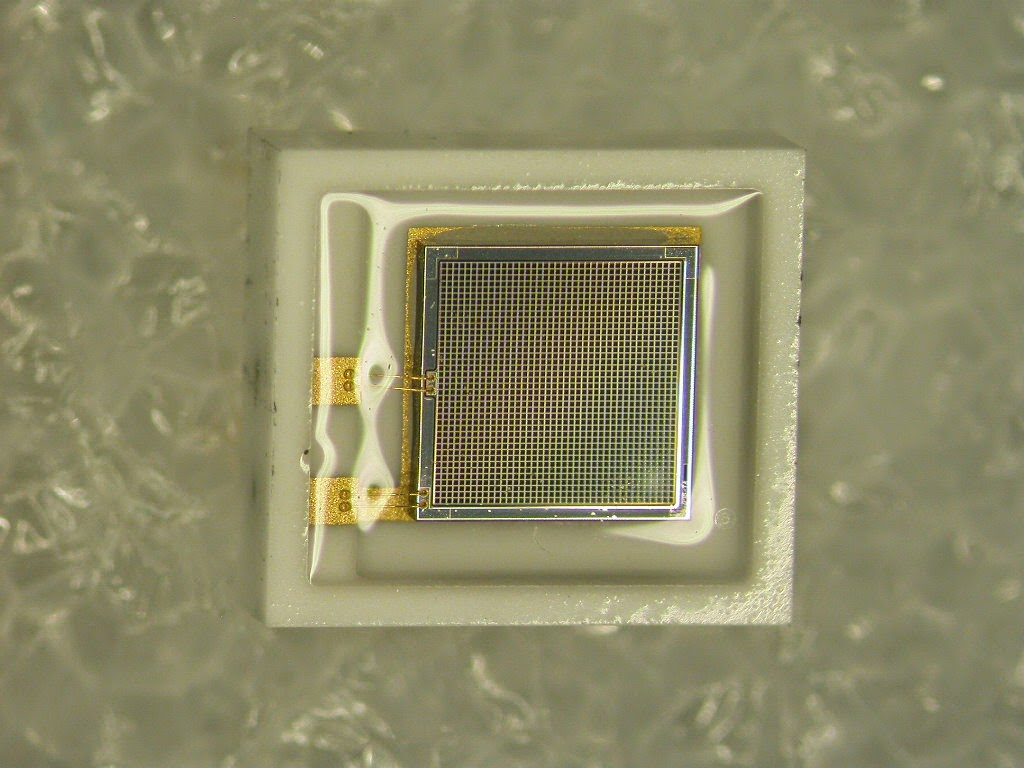
\includegraphics[scale=0.20]{imm/lct4_1.jpg}
\end{center}
\caption{Image of LCT4/9 taken through a microscope.}
\label{fig:lct4_1}
\end{figure}

This set of MPPCs produced by Hamamatsu, have an included proprietary circuit board with power supply for a direct hardware control from PC via USB connection (see Fig~\ref{fig:mppc}).\\
The C12332 is a simple evaluation starter kit for non-cooled MPPC. MPPC evaluation is possible by mounting an MPPC in the socket of the sensor circuit board. The power supply circuit board is equipped with the C11204-01, a high-accuracy, high-voltage power supply that provides the operating voltage from MPPC. It operates just by connecting to an extenal power supply ($\pm 5V$). It is also equipped with a USB interface that can be used to set the operating voltage and temperature compensation coefficient from a PC running the supplied sample software.\\
We used the power supply circuit board with serial number C12332 with nominal gain of 21 for LCT4/9.\\

\begin{figure}[!h]
\begin{center}
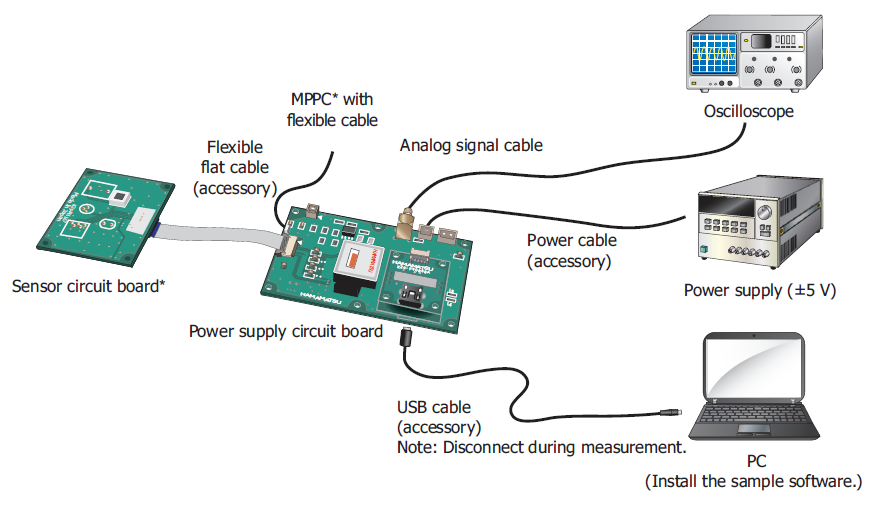
\includegraphics[scale=0.5]{imm/mppc.png}
\end{center}
\caption{Connection example}
\label{fig:mppc}
\end{figure}

Sensor circuit and power supply board have been both fixed on an aluminum support covered by black duct tape (Fig~\ref{fig:mppc2}).
\begin{figure}[!h]
\begin{center}
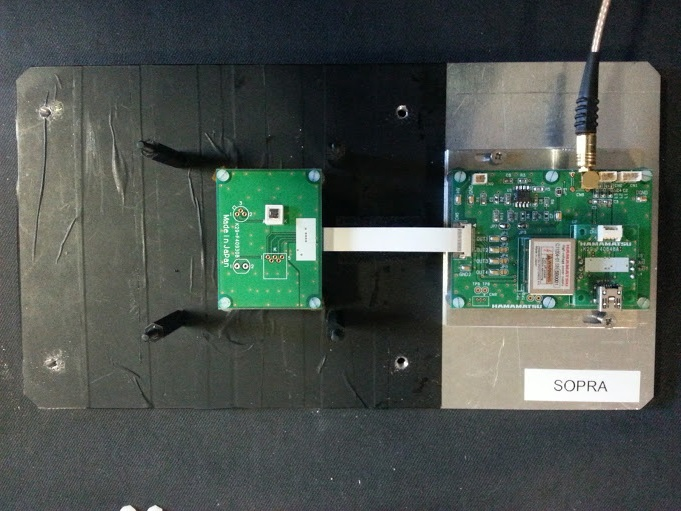
\includegraphics[scale=0.5]{imm/mppc2.jpg}
\end{center}
\caption{Circuit and sensor boards on support}
\label{fig:mppc2}
\end{figure}

The GAGG rod has been placed over a single SiPM. The extremity of the rod in contact with the SiPM window entrance has been covered with optical grease in order to improve the transmission of optical photons to the microcells.\\
A dedicated support has been projected and realized specifically for this experiment in order to hold the rod under study and to guarantee its contact with the SiPM.\\
The project drawing is reported in Fig~\ref{fig:cad} and the principal components legend below:
\begin{itemize}
\item (1) Aluminum support
\item (2) secondary mobile support for power supply circuit board
\item (4) dark box
\item (6-7) support columns 
\item (8) support for rod-stops
\item (9) rod stops
\item (11) circular support for x-ray sources
\end{itemize}
The produced support inserted in the experimental set-up is shown in Fig~\ref{fig:support1}.

\newpage
\begin{figure}[!h]
\begin{center}
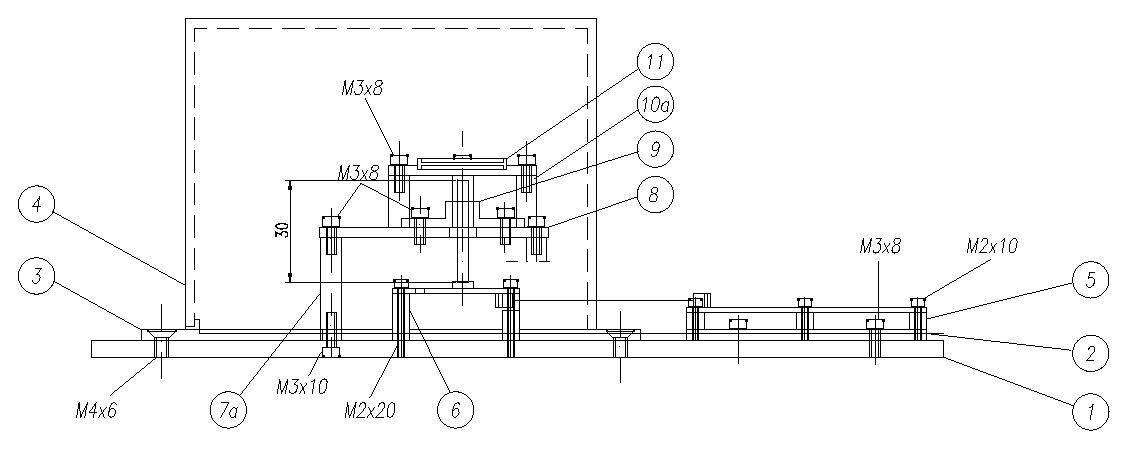
\includegraphics[scale=0.45]{imm/cad1.png}\\
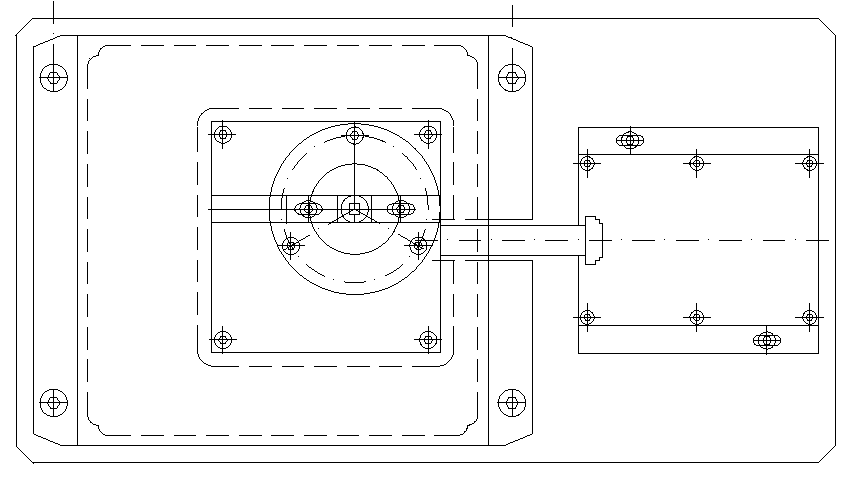
\includegraphics[scale=0.45]{imm/cad2.png}\\
\end{center}
\caption{Front and side projection of entire setup.}
\label{fig:cad}
\end{figure}

\begin{figure}[!h]
\begin{center}
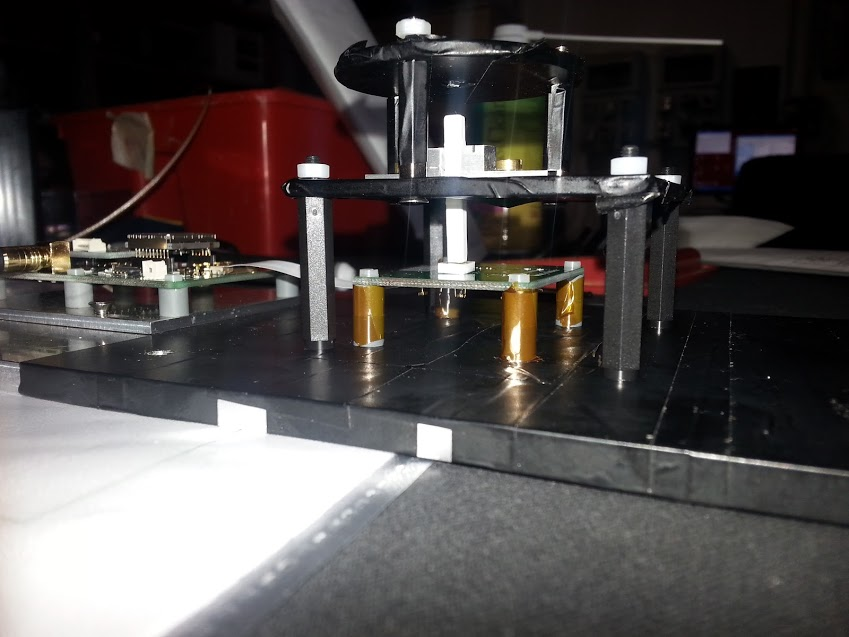
\includegraphics[scale=0.28]{imm/support1.jpg}
\end{center}
\caption{Built setup}
\label{fig:support1}
\end{figure}
\newpage
Sources of $^{241}Am$, $^{109}Cd$, $^{133}Ba$, $^{55}Fe$, $^{137}Cs$ have been used to illuminate the rod, placed at a distance of about $5mm$ from the rod top, put on a circular aluminum support designed for the used radioactive sources (Fig.~\ref{fig:support1}). The source, produced by \emph{Eckert \& Ziegler} company, has a diameter of $3mm$ (Fig~\ref{fig:source}). It's flux has not been collimated.\\

\begin{figure}[!h]
\begin{center}
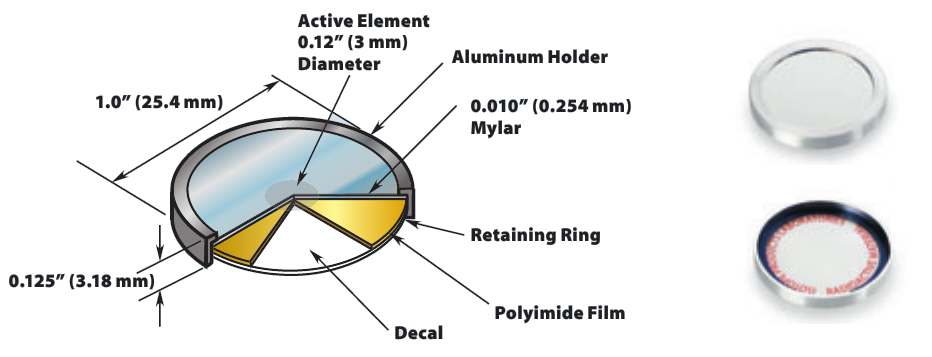
\includegraphics[scale=0.4]{imm/source.png}
\end{center}
\caption{Type M disk used as x-rays source~\cite{instr:sou}. }
\label{fig:source}
\end{figure}

The alignment of the source along Z-direction has been carried out optically because the diameter of the beam spot was larger than the rod one, and therefore a rough alignment was sufficient.\\
The SiPM signal was read and processed by electronic chain whose diagram is reported in Fig~\ref{fig:el_scheme}. Power supply circuit board permitted to vary the operative voltage applied to the SiPM through USB connection and thus the SiPM internal gain.\\
The signal from SiPM was processed by a pre-amplifier welded on Hamamatsu circuit board and an amplifier ORTEC 450 \emph{Research Amplifier}, and then digitized by a Multi-Channel Analyzer (MCA) Amptek 8000A, which splits signal into 1024 digital channels in a dynamic range of 0-5V or 0-10V.\\
The SiPM is very sensitive to visible light, therefore dark conditions are needed to perform the measurements. The dark conditions were assured by a \emph{dark box} ((4) in Fig~\ref{fig:cad}), a carton and a black cloth placed over the set-up.

\begin{figure}[!h]
\begin{center}
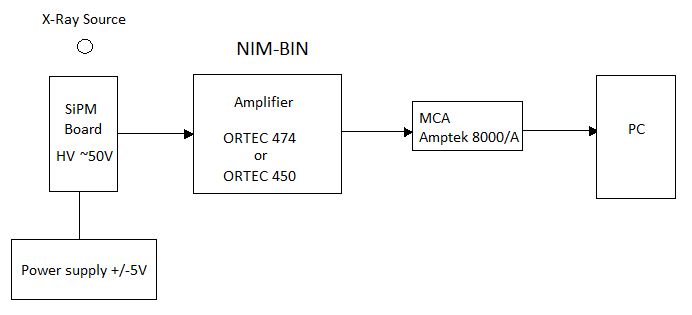
\includegraphics[scale=0.55]{imm/chain.png}
\end{center}
\caption{Sketch scheme of the electronic chain employed in the measurements to read and store SiPM signals}
\label{fig:el_scheme}
\end{figure}
\newpage
\section{Definition of the operative range}
\subsection{Set-up parameters}
Some preliminary operations must be performed before starting the measurement process. In particular, the parameters of the electronic chain must be set to proper values, the digital channels of the MCA must be converted into charge values through a calibration and the experimental conditions must be analyzed.\\[2ex]
The gains of the used SiPM and amplifier can be varied. It has been necessary to properly set these parameters in order to generate a signal within a range suitable to the MCA input dynamics.\\
During the adjusting process, the gains were changed until the whole signal from the SiPM has been included in the spectrum collected by the MCA. An intense light source was necessary to guarantee a high measurement rate in order to collect a suitable number of events in a short time and to dominate dark current.\\
We know that our GAGG rod has a light yield of $\sim 60$ photons/keV ~\cite{gagg:1} and the activity of the $^{241}Am$ is $\sim 10\mu Ci$.\\[2ex]
Here the instruments limitations:
\begin{itemize}
\item Hamamatsu datasheets says that we have a linearity of signal when we illuminate at the same time a number $<40\%-50 \%$ of MPPC pixels.
\item MPPC signals are very fast ($<100ns$) and very frequents, but MCA accepts a minimum shaping time of $250ns$ with a 'first peak detection'.
\end{itemize}
In order to prevent saturations or non-linearity in the final spectrum, we chose set-up parameters so that $^{241}Am$ photo-peak @ $59.5 keV$ was placed in the middle of MCA dynamic range.\\
Gain and integration time of ORTEC450 and \emph{operative tension} ($V_{op}$) of SiPMs have been changed to optimize quality of spectrum.

\subsection{Expected efficiency}
To define an energy range of measurement system we needed to know maximum efficiency interval for scintillator rod, SiPMs and both.
Detector efficiency, as function of energy, is defined by:
\begin{equation}
\epsilon(E) = T(E)\cdot A(E)
\end{equation}
where T(E) and A(E) are respectively (\ref{eqn:t}) transparency (\ref{eqn:a}) and absorption with respect to energy radiation.

\begin{equation}
\label{eqn:t}
T(E) = e^{-\rho \delta \sigma(E)}
\end{equation}

\begin{equation}
\label{eqn:a}
A(E) = 1 - e^{-\rho \delta \sigma(E)}
\end{equation}

$\rho$ is the material density, $\delta$ the thickness and $\sigma(E)$ the cross section sums for coherent/incoherent Compton scattering and photoelectric effect as a function of energy. Plotted results are showed in Fig~\ref{fig:eff_gagg}.\\
From literature I have found the SiPMs quantum efficiency curve~\cite{bonanno:1} and the GAGG light emission~\cite{gagg:3} to calculate the total efficiency of SiPM+GAGG system (Eq \ref{eqn:e}).

\begin{figure}[!h]
\begin{center}
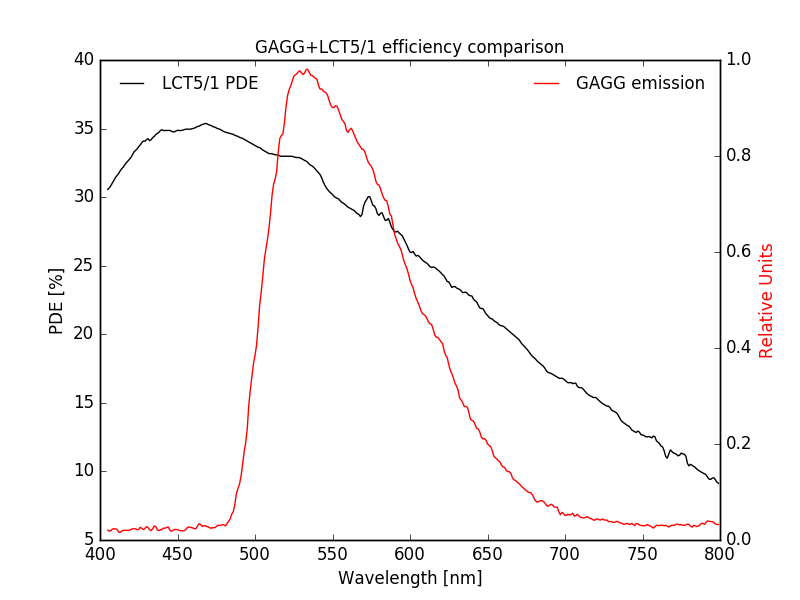
\includegraphics[scale=0.4]{imm/lct_gagg.png}
\end{center}
\caption{LCT5/1 QE and GAGG light emission}
\label{fig:lin1}
\end{figure}

\begin{equation}
\epsilon_{tot} = \frac{\int_{\lambda} d\lambda \epsilon_{SiPM} \cdot \epsilon_{GAGG} }{\int_{\lambda} d\lambda \epsilon_{GAGG} }
\label{eqn:e}
\end{equation}

Calculated efficiencies for LCT4/9 and LCT5/1 are listed in Tab~\ref{tab:eff}.

\begin{table}[h]
\begin{tabular}{cc}
\toprule
SiPM & Tot. efficiency \\
\midrule
LCT4/9 + GAGG& 30.1\% \\
LCT5/1 + GAGG& 28.7\% \\
\bottomrule
\end{tabular}
\caption{SiPM+GAGG efficiency}
\label{tab:eff}
\end{table}

\section{Circuit calibration with X-ray sources}
I calibrated the electronic chain has been in order to convert the digital channels of the MCA output spectra in charge values.\\
Signals with similar amplitude, rise time and fall time of SiPM was produced by a pulse generator (BNC BL-2).\\
I measured the exact values of applied voltages through an oscilloscope connected to circuit. At the same time, the channel number of the peak produced by the signal in the MCA spectrum was stored and associated with the applied voltage.\\
This operation has been repeated for different $V_{op}$ (Fig~\ref{fig:lin1}).

\begin{figure}[!h]
\begin{center}
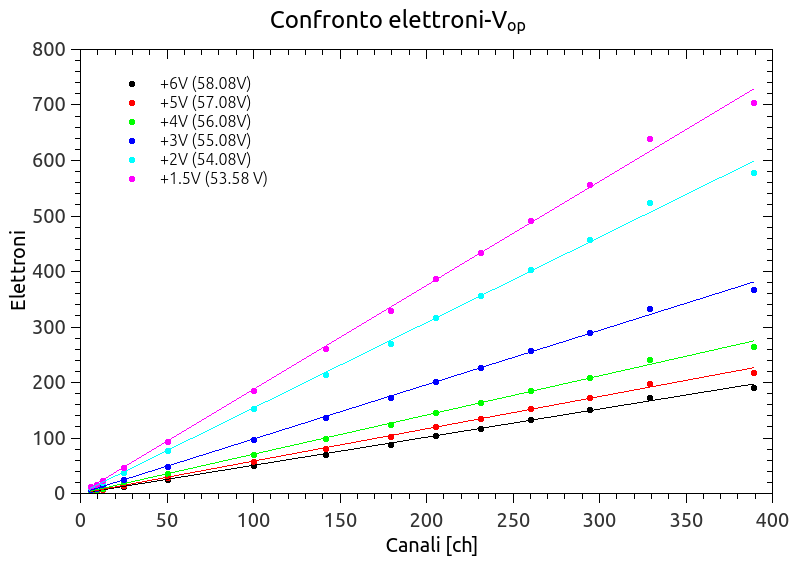
\includegraphics[scale=0.4]{imm/confronto_tot.png}
\end{center}
\caption{Linear calibration function used to convert the measured digital channels into charge values for LCT5/1.}
\label{fig:lin1}
\end{figure}
Furthermore an energy calibration was performed with radioactive sources described in section 1.1 (Fig~\ref{fig:lin}).\\
I selected a gaussian model to fit sources photo-peaks.
In order to improve fit, I studied a model that explain photopeak asymmetries for $^{109}Cd$ and $^{133}Ba$ (Fig~\ref{fig:th}).

\begin{figure}[!h]
\begin{center}
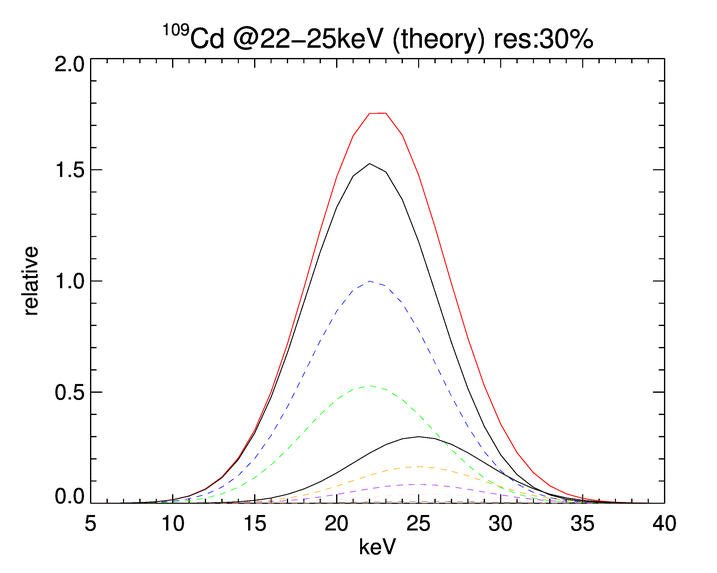
\includegraphics[scale=0.2]{imm/22kev_gauss.png}
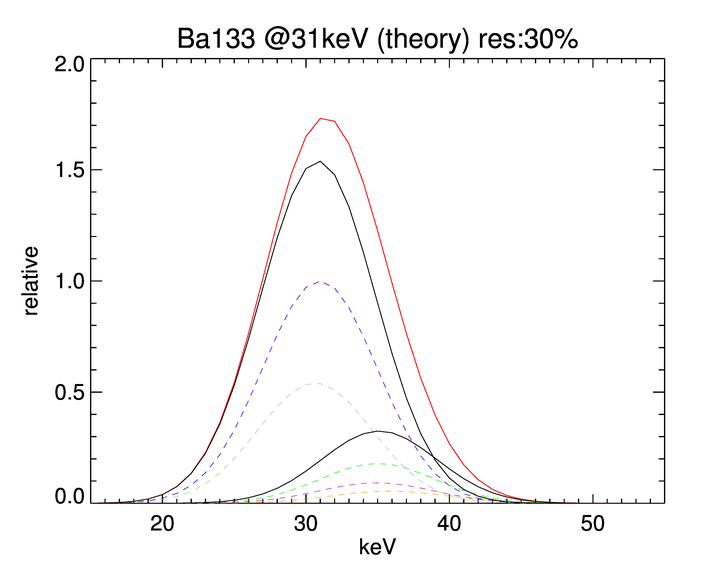
\includegraphics[scale=0.2]{imm/31kev_gauss.png}
\end{center}
\caption{Theoretical model that assumes laboratory probability of each convoluted line for a resolution of 30\%. Data from XCOM.}
\label{fig:th}
\end{figure}

\begin{figure}[!h]
\begin{center}
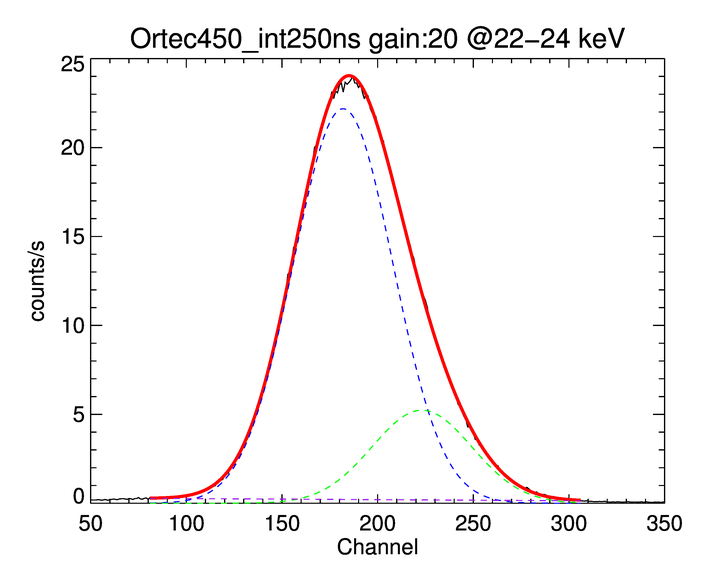
\includegraphics[scale=0.19]{imm/cd.png}
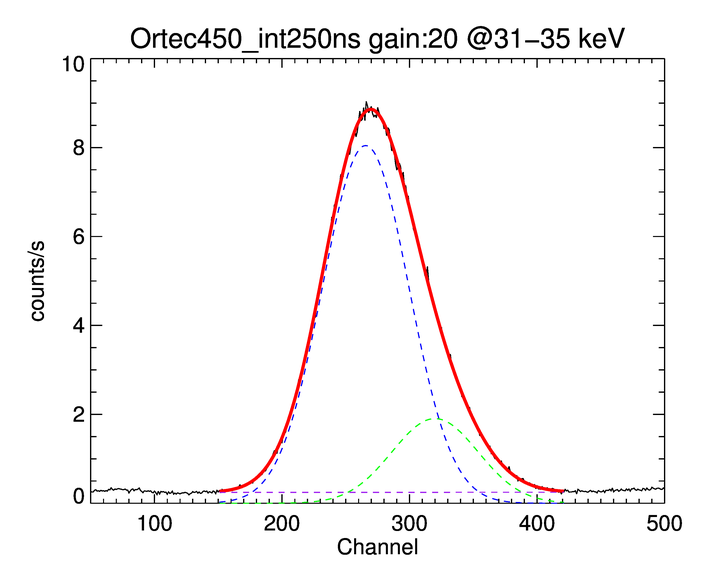
\includegraphics[scale=0.19]{imm/ba.png}
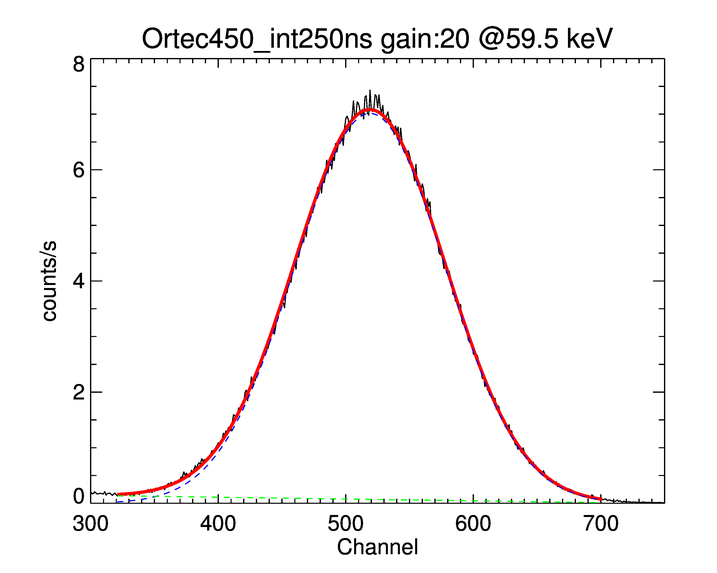
\includegraphics[scale=0.19]{imm/am.png}
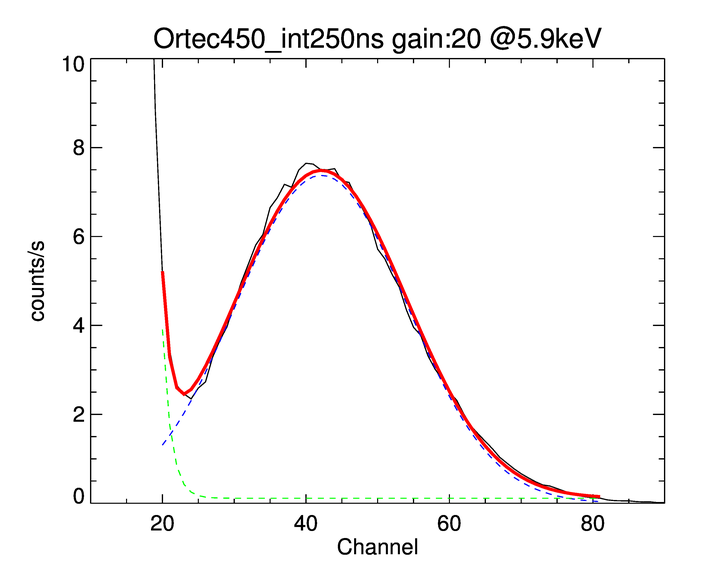
\includegraphics[scale=0.19]{imm/fe.png}
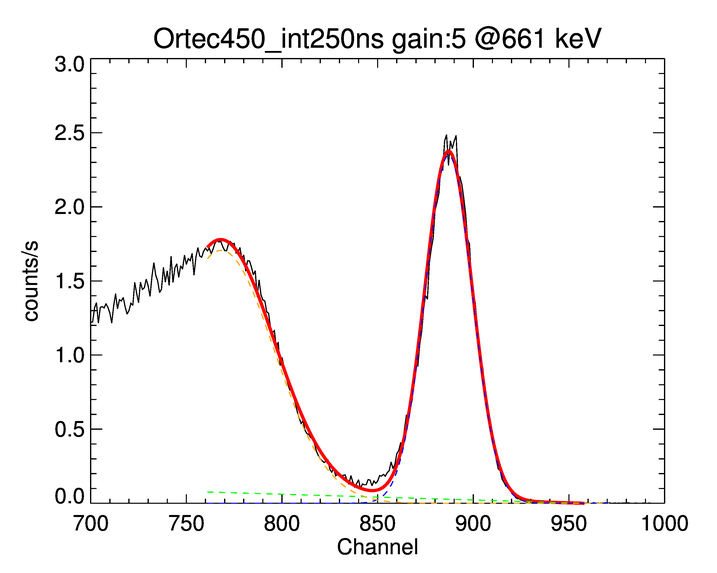
\includegraphics[scale=0.19]{imm/cs.png}
\end{center}
\caption{To left to right respectively: $^{109}Cd$ @ 22keV, $^{133}Ba$ @ 31keV, $^{241}Am$ @ 59.5keV, $^{55}Fe$ @ 5.9 kev, $^{137}Cs$ @ 661 keV} 
\label{fig:fit}
\end{figure}

\begin{figure}[!h]
\begin{center}
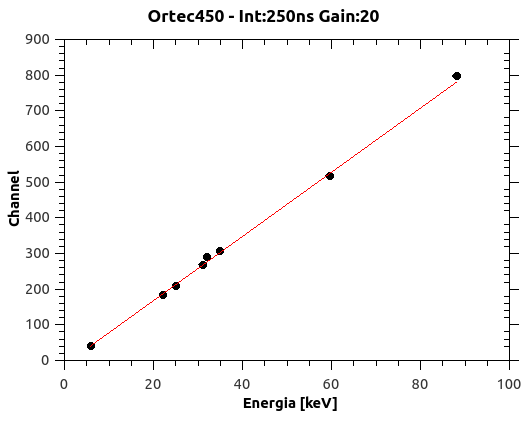
\includegraphics[scale=0.45]{imm/lin.png}
\end{center}
\caption{Linear energy calibration in the range of 0-90KeV for LCT4/9.}
\label{fig:lin}
\end{figure}

We also detected non-linearity for high energies values as expected (Fig~\ref{fig:nl}).
\begin{figure}[!h]
\begin{center}
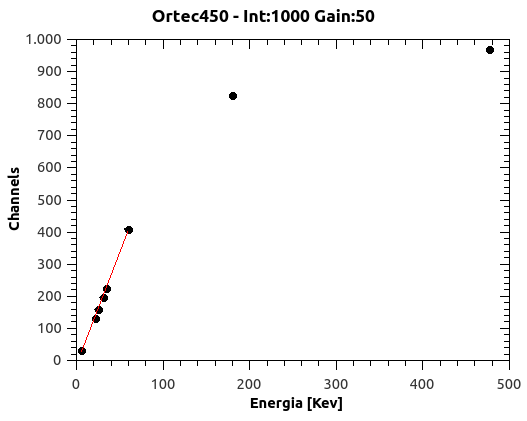
\includegraphics[scale=0.5]{imm/1000_50_fit.png}
\end{center}
\caption{Non-linearity detection at high energies with LCT4/9.}
\label{fig:nl}
\end{figure}
\newpage
\subsection{Dark/Background noise}
Background noise spectra (Fig~\ref{fig:fondo}) are fundamental informations to select best configuration for acquiring data.\\
A study of \emph{dark} counts has been performed to understand behavior of SiPM as $V_{op}$ changes.

\begin{figure}[!h]
\begin{center}
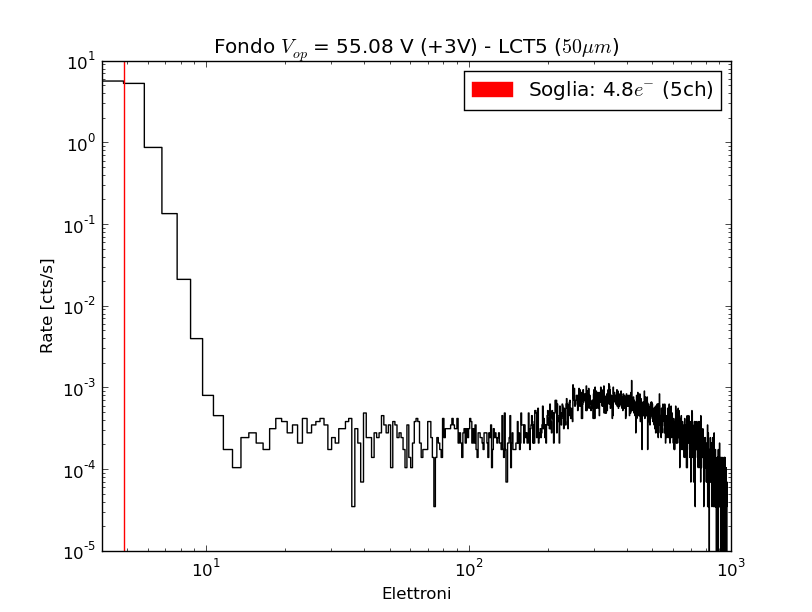
\includegraphics[scale=0.5]{imm/fondo.png}
\end{center}
\caption{Background noise acquisition with LCT5/1 ($V_{op}=+3V$)+ GAGG.}
\label{fig:fondo}
\end{figure}

Environmental noise is negligible with respect to sources rate. At low charge collection dark current dominates.\\
An exponential curve was chosen to fit dark noise (Fig~\ref{fig:noise}). 

\begin{figure}[!h]
\begin{center}
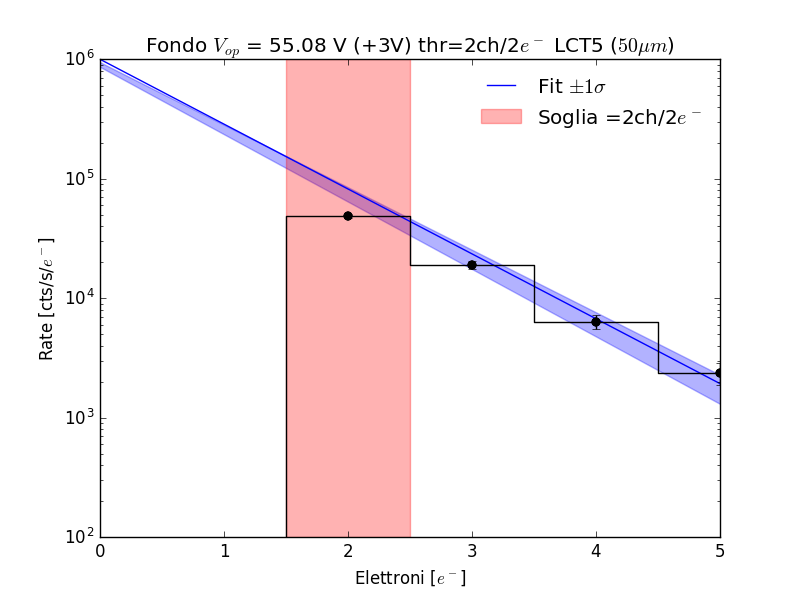
\includegraphics[scale=0.25]{imm/fit3_2.png}
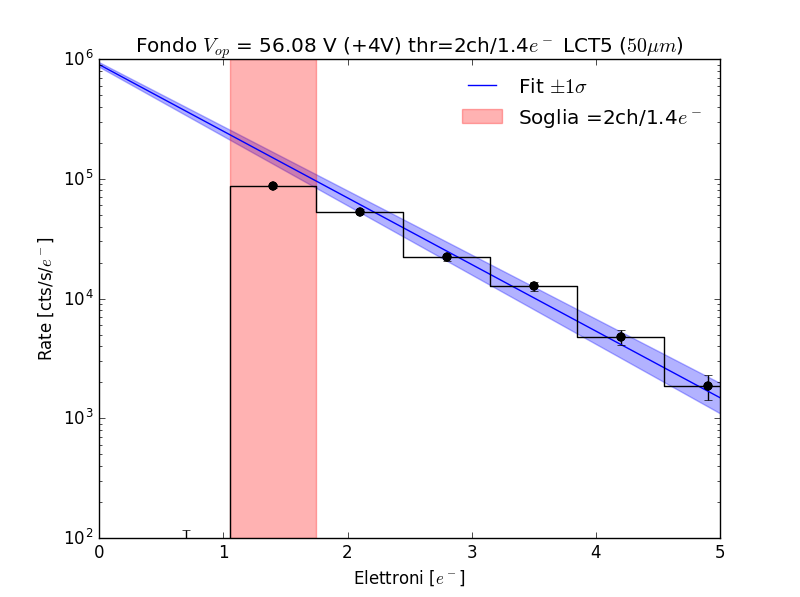
\includegraphics[scale=0.25]{imm/fit4_2.png}
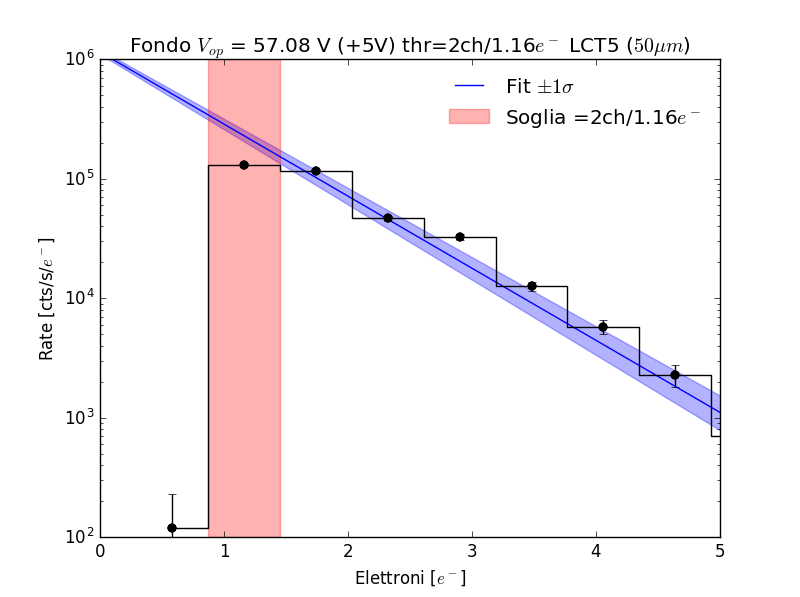
\includegraphics[scale=0.25]{imm/fit5_2.png}
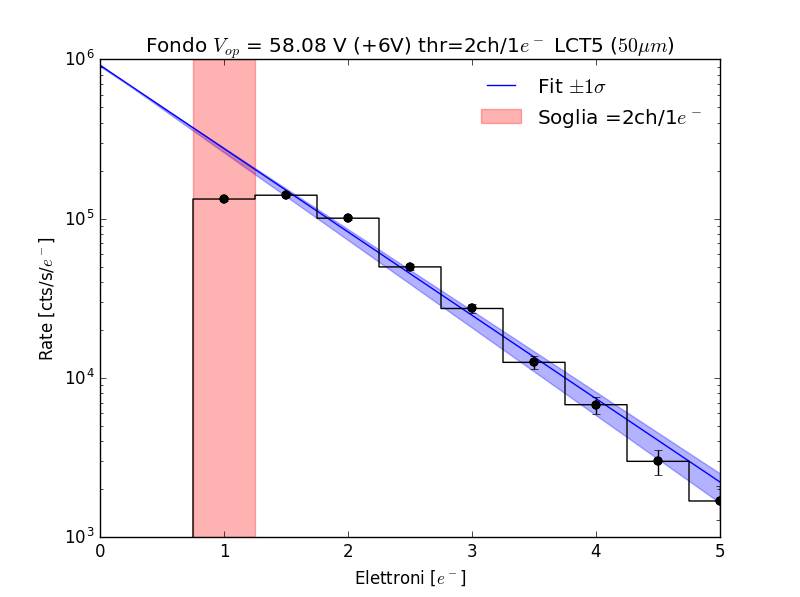
\includegraphics[scale=0.25]{imm/fit6_2.png}
\end{center}
\caption{Dark rate study for LCT5/1+ GAGG} 
\label{fig:noise}
\end{figure}


\section{Energy resolution measurement}
Fitted sources photopeaks of section 1.3 has been analyzed to extrapolate energy resolution as a function of $V_{op}$.\\
We note that dark rate increases with the increase of $V_{op}$ but resolution seems to be better (decreases) with $V_{op}$.\\
Left plot of Fig~\ref{fig:res} ($^{55}Fe$ @ 5.9 kev), has an irregular distribution with respect to $^{241}Am$ case, due to nearness of dark noise that affects error of photopeak position and width. 

\begin{figure}[!h]
\begin{center}
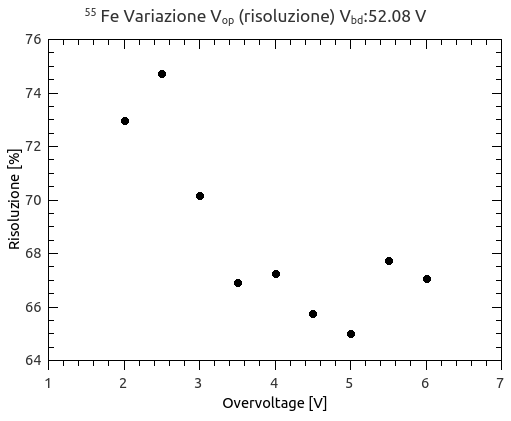
\includegraphics[scale=0.35]{imm/resfe.png}
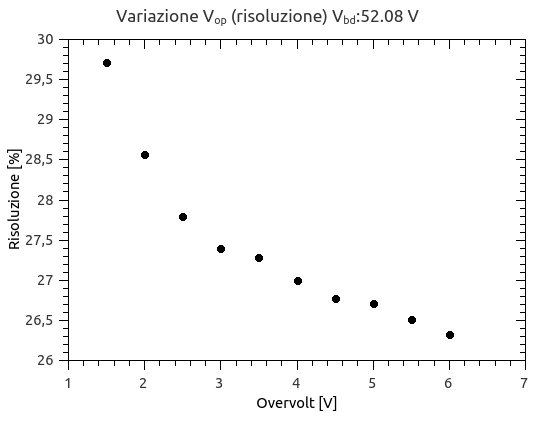
\includegraphics[scale=0.35]{imm/resam.png}
\end{center}
\caption{Resolution for $^{55}Fe$ peak (left) and ($^{241}Am$) peak as function of $V_{op}$.} 
\label{fig:res}
\end{figure}

\chapter{Scatterer characterization}
Scatterer rods are the inner components of Compton polarimeter design. They are made of plastic scintillator  
Plastic scintillators have a low atomic number $Z$.\\
<<<<<<< HEAD
=======
Ciao
>>>>>>> master

\section{Scatterer properties}

\section{Study at low energy}
\subsection{Set-up parameters}
\subsection{Dark current}

\section{Study at high energy}
\subsection{Set-up parameters}
\subsection{Spectra analysis}
\subsection{Energy resolution measurement}


\clearpage
\addcontentsline{toc}{chapter}{\refname}
\begin{thebibliography}{20}

\bibitem{abs:1}
Hye-Lim Kim et al. Journal of Ceramic Processing Research. Vol. 16, No. 1, pp. 124-128, 2015

\bibitem{gagg:1}
\emph{Ce:GAGG Scintillator Crystal}, datasheet from Furukawa website (\url{http://www.furukawa-denshi.co.jp/cgi-bin/pdfdata/20140428162950.pdf})

\bibitem{gagg:2}
\emph{XCOM: Photon Cross Sections Database \url{http://www.nist.gov/pml/data/xcom/}}

\bibitem{instr:sou}
\emph{Section Gamma and X-Ray Standards. \url{http://www.ezag.com/fileadmin/ezag/user-uploads/isotopes/isotopes/Isotrak/isotrak-pdf/Product_literature/EZIPL/Gamma_Standards_All_Types.pdf}}

\bibitem{bonanno:1}
Bonanno et al. doi:10.1016/j.nima.2015.10.064

\bibitem{gagg:3}
Seferis et al. doi:10.1007/978-3-319-00846-2-113, 2013


\end{thebibliography}
\end{document}
